\appendix
\addtocontents{toc}{%
  \protect\vspace{1em}%
  \protect\noindent \bfseries \appendixtocname\protect\par
  \protect\vspace{-.5em}%
 }
 \renewcommand{\chaptername}{\appendixname}

\begin{appendices}

\chapter{Appendix A}

\section{Socket.IO Implementation Script}
\label{server:socket}

\begin{lstlisting}[caption={socket.js on Application Server},label={code:server_socket}]
SocketManager.prototype.listen = function(server){
  ...
  io = socketio.listen(server);
  io.sockets.on('connection', _handlerSocket);
  _handlerSip();
}

function _handlerSocket(socket) {
  var delivery = dl.listen(socket);
    ...
  socket.on('sip',function (data){
    switch(data.type){
      case 'register':
        if(data.username != ""){
          gw.register(data.content.browserClient,function(result){
            socket.emit('sip',result);
          });
        }
        break;
      ...
    }
  });

  socket.on('webrtc', function (data) {
        ...  
    });

  socket.on('message',function(data){
    ...
  });

  socket.on('disconnect', function() {
    ...
  });

  delivery.on('receive.success',function(file){
    ...
    fs.writeFile(file.name,file.buffer, function(err){
      if(err){
        console.log('File could not be saved.');
      }else{
        console.log('File saved.');
        _und.each(clients,function(client,key){
          if(sendingClient.conf_id && client.conf_id == sendingClient.conf_id && client.username != sendingClient.username){
            ...
            client.delivery.send({
              name: file.name,
              path : './' + file.name
            });

          }
        });

        fs.unlink('./' + file.name);
      };
    });
  });

}
\end{lstlisting}

\section{SIP Implementation Script}
\label{server:sip}

\begin{lstlisting}[caption={sip.js on Application Server},label={code:sipjs}]
util.inherits(SipGateway, EventEmitter);
...
function createRegister(user){
	return {
	  method: 'REGISTER',
	  uri: 'sip:' + user.hostname,
	  headers:
	  {
	  	'call-id': user.callid,
	  	cseq: {method: 'REGISTER', seq: ++user.seq},
	  	from: {name: '', uri: 'sip:' + user.name + '@' + user.hostname, params: { tag: user.tag }},
	    to: {name: '', uri: 'sip:' + user.name + '@' + user.hostname},
	    expires: 3600,
	  	contact:  [{
      	uri: 'sip:' + user.name + '@'+ hostPublicAddress + ':' + hostPort
      }]

	  }
	}
}
function createInviteACK(rs,client,sdp){
	var uri = rs.headers.contact[0].uri.split(';');
	if(uri[0].split(':').length != 3){
		uri[0] = uri[0] + ':5060';
	}
	...
}
...
SipGateway.prototype.init = function () {
	...
	registry = {};
	sip.start({
		port: hostPort,
	  logger: {
	    ...
	  },
	  publicAddress: hostPublicAddress,
	  tcp: false
	},
	function(rq) {
	  try {
	    if(rq.method === 'REGISTER') {
	      ...
	    }
	    else if(rq.method === 'INVITE') {
	      ...
	      var rs = sip.makeResponse(rq, 100, 'Trying');
	      sip.send(rs);
	      if(contact) {
	      	...
	        self.emit('SIPREMOTE',{
	        	type: 'INVITE',
	        	content:{
	        		fromNumber: sip.parseUri(rq.headers.from.uri).user,
	        		toNumber: username,
	        		inviteRequest: rq
	        	}
	        });
	      }
	      ...
	});
}
function _register(client,callback){
	var rq = createRegister(client);
	sip.send(rq,function(rs){
		if(rs.status === 401){
			var user = client;
			var creds = { user: user.name, password: user.password, realm: user.hostname };
			rq.headers['cseq'].seq++;
	    ...
	    digest.signRequest(creds, rq, rs, creds);
			sip.send(rq,function(rs){
				if(rs.status === 200){
					client.authorization = rq.headers.authorization;
					if(!client.registerTimer){
						client.registerTimer = setInterval(function(){
							console.log('register timer');
							_register(client);
						},parseInt(rs.headers.expires)*1000);
					}
                    ...
				}else{
					...
				}
			});
		}else if(rs.status === 200){
			...
		}
	});
}
SipGateway.prototype.register = function(client,callback){
    ...
	_register(registry[client.name],callback);
}
...
module.exports.SipGateway = SipGateway;
\end{lstlisting}


\section{XMS Implementation Script}
\label{server:xms}

\begin{lstlisting}[caption={xms.js on Application Server},label={code:xms}]
XmsManager.prototype.createXMSCall = function(data,callback){
  var requestContent = "<web_service version=\"1.0\">";
  ...
  if(data.callType === 'webrtc'){
    requestContent += " encryption=\"dtls\"" + " ice=\"yes\"";
  }
  ...
  var req = http.request({
    host: xmsAddress,
    port: xmsPort,
    method: 'POST',
    path: xmsPath + 'calls?appid=' + xmsAppId,
    headers: {
      'Accept' : 'application/xml',
      'Content-Type' : 'application/xml',
      'Content-Length' : requestContent.length
    }
  }, function(res) {
    var resData = '';
    res.setEncoding('utf8');
    res.on('data', function (chunk) {
      resData += chunk;
    }).on('end', function() {
      if(resData != ''){
        xmlparser.parseString(resData,function(err,result){
          var xmsSdp = result['web_service']['call_response'][0]['$'].sdp;
          var id = result['web_service']['call_response'][0]['$'].identifier;
          var regex = new RegExp(xmsAddress,"g");
          pub_xmsSdp = xmsSdp.replace(regex,xmsPublicAddress);
          callback(pub_xmsSdp.replace(/\n/g,"\r\n"),id);
        });
      }
    });
  });
  req.write(requestContent);
  req.end();
}
...
module.exports.XmsManager = XmsManager;
\end{lstlisting}

\section{MSG Implementation Script}
\label{server:msg}

\begin{lstlisting}[caption={msg.js on Application Server},label={code:msg}]
MsgManager.prototype.login = function(loginDto,success,fail){

	var loginStr = JSON.stringify(loginDto);

	var options = {
		host: msgRestUrl,
		path: '/your/url/here/loginWithDto',
		method : 'POST',
		headers: {
			"Accept" : "application/json",
			"Content-Type" : "application/json",
			'Content-Length' : loginStr.length
		}
	};

	var req = https.request(options, function(res) {
		var resData = '';
	  console.log("MSG:LOGIN:statusCode: ", res.statusCode);
	  console.log("MSG:LOGIN:headers: ", res.headers);
	  res.setEncoding('utf8');

	  res.on('data', function (chunk) {
      resData += chunk;
    }).on('end', function() {
    	if(resData != ''){
    		var jsonObject = JSON.parse(resData);
    		if(jsonObject.code === 200){
    			success(jsonObject,res.headers['set-cookie'][0]);
    		}else{
    			fail(jsonObject);
    		}
    	}
    });
	});

	req.write(loginStr);
	req.end();

	req.on('error', function(e) {
	  console.error(e);
	  fail(e);
	});

}

MsgManager.prototype.sendSMS = function(organization,login,cookie,msgObj,success,fail){

	var msgStr = JSON.stringify(msgObj);
	console.log(msgObj);

	var options = {
		host: msgRestUrl,
		path: '/your/url/here/sms',
		method : 'POST',
		headers : {
			"Accept" : "application/json",
			"Content-Type" : "application/json",
			"organization" : organization,
			"login" : login,
			"Cookie" : cookie,
			'Content-Length' : msgStr.length
		}
	};

	var req = https.request(options, function(res) {
		var resData = '';
	  console.log("MSG:SENDSMS:statusCode: ", res.statusCode);
	  console.log("MSG:SENDSMS:headers: ", res.headers);
	  res.setEncoding('utf8');

	  res.on('data', function (chunk) {
      resData += chunk;
    }).on('end', function() {
    	if(resData != ''){
    		var jsonObject = JSON.parse(resData);
    		console.log('MSG:SENDSMS:jsonObject:',jsonObject);
    		if(jsonObject.code === 200){//TODO: check report values as true
    			success();
    		}else{
    			fail();
    		}
    	}
    });
	});

	req.write(msgStr);
	req.end();

	req.on('error', function(e) {
	  console.error(e);
	  fail();
	});

}

module.exports.MsgManager = MsgManager;
\end{lstlisting}

\chapter{Appendix C}

\section{WebRTC in Dart}
\label{research:dart_webrtcctrl}

\begin{lstlisting}[caption={WebRTCCtrl in Dart application client},label={code:dart_webrtcctrl}]
library webRTCCtrl;

import 'package:angular/angular.dart';
import 'dart:html';
import 'package:webrtcDemo/speaker/speack_client.dart';

@NgController(
  selector : '[webrtc-ctrl]',
  publishAs : 'ctrl'
)

class WebRTCCtrl {

  static const String SERVER_URL = "ws://127.0.0.1:3001";

  String websocketUrl = SERVER_URL;

  WebRTCCtrl() {
    _initConnection();
  }

  void _initConnection(){
    var speaker = new SpeakerClient(websocketUrl, room: 'room');

    speaker.createStream(audio: true, video: true ).then((stream) {
      var video = new VideoElement()
        ..autoplay = true
        ..src = Url.createObjectUrl(stream);

      document.body.append(video);
    });

    speaker.onAdd.listen((message) {
      var video = new VideoElement()
        ..id = 'remote${message['id']}'
        ..autoplay = true
        ..src = Url.createObjectUrl(message['stream']);

      document.body.append(video);
    });

    speaker.onLeave.listen((message) {
      document.query('#remote${message['id']}').remove();
    });
  }
}
\end{lstlisting}

\chapter{Appendix D}

\section{AngularJs Files Structure}
\label{code:angularjs_structure}

\begin{figure}
	\centering
    	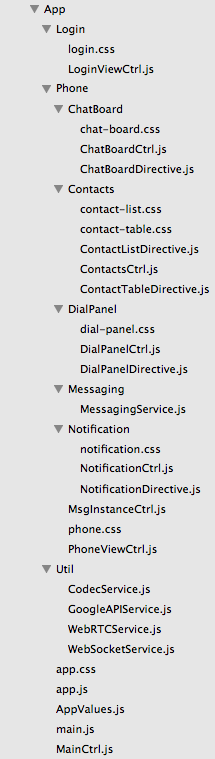
\includegraphics[height=0.45\textheight,natwidth=610,natheight=642]{figs/angularjs_structure.png}
  	\caption{Prototype Application AngularJs Files}
  	\label{fig:angularjs_structure}
\end{figure}

\end{appendices}
